% Options for packages loaded elsewhere
\PassOptionsToPackage{unicode}{hyperref}
\PassOptionsToPackage{hyphens}{url}
\documentclass[
  12pt,
]{article}
\usepackage{xcolor}
\usepackage[margin=1in]{geometry}
\usepackage{amsmath,amssymb}
\setcounter{secnumdepth}{-\maxdimen} % remove section numbering
\usepackage{iftex}
\ifPDFTeX
  \usepackage[T1]{fontenc}
  \usepackage[utf8]{inputenc}
  \usepackage{textcomp} % provide euro and other symbols
\else % if luatex or xetex
  \usepackage{unicode-math} % this also loads fontspec
  \defaultfontfeatures{Scale=MatchLowercase}
  \defaultfontfeatures[\rmfamily]{Ligatures=TeX,Scale=1}
\fi
\usepackage{lmodern}
\ifPDFTeX\else
  % xetex/luatex font selection
  \setmainfont[]{Times New Roman}
  \setmonofont[]{Courier New}
\fi
% Use upquote if available, for straight quotes in verbatim environments
\IfFileExists{upquote.sty}{\usepackage{upquote}}{}
\IfFileExists{microtype.sty}{% use microtype if available
  \usepackage[]{microtype}
  \UseMicrotypeSet[protrusion]{basicmath} % disable protrusion for tt fonts
}{}
\usepackage{setspace}
\makeatletter
\@ifundefined{KOMAClassName}{% if non-KOMA class
  \IfFileExists{parskip.sty}{%
    \usepackage{parskip}
  }{% else
    \setlength{\parindent}{0pt}
    \setlength{\parskip}{6pt plus 2pt minus 1pt}}
}{% if KOMA class
  \KOMAoptions{parskip=half}}
\makeatother
\usepackage{color}
\usepackage{fancyvrb}
\newcommand{\VerbBar}{|}
\newcommand{\VERB}{\Verb[commandchars=\\\{\}]}
\DefineVerbatimEnvironment{Highlighting}{Verbatim}{commandchars=\\\{\}}
% Add ',fontsize=\small' for more characters per line
\newenvironment{Shaded}{}{}
\newcommand{\AlertTok}[1]{\textcolor[rgb]{1.00,0.00,0.00}{\textbf{#1}}}
\newcommand{\AnnotationTok}[1]{\textcolor[rgb]{0.38,0.63,0.69}{\textbf{\textit{#1}}}}
\newcommand{\AttributeTok}[1]{\textcolor[rgb]{0.49,0.56,0.16}{#1}}
\newcommand{\BaseNTok}[1]{\textcolor[rgb]{0.25,0.63,0.44}{#1}}
\newcommand{\BuiltInTok}[1]{\textcolor[rgb]{0.00,0.50,0.00}{#1}}
\newcommand{\CharTok}[1]{\textcolor[rgb]{0.25,0.44,0.63}{#1}}
\newcommand{\CommentTok}[1]{\textcolor[rgb]{0.38,0.63,0.69}{\textit{#1}}}
\newcommand{\CommentVarTok}[1]{\textcolor[rgb]{0.38,0.63,0.69}{\textbf{\textit{#1}}}}
\newcommand{\ConstantTok}[1]{\textcolor[rgb]{0.53,0.00,0.00}{#1}}
\newcommand{\ControlFlowTok}[1]{\textcolor[rgb]{0.00,0.44,0.13}{\textbf{#1}}}
\newcommand{\DataTypeTok}[1]{\textcolor[rgb]{0.56,0.13,0.00}{#1}}
\newcommand{\DecValTok}[1]{\textcolor[rgb]{0.25,0.63,0.44}{#1}}
\newcommand{\DocumentationTok}[1]{\textcolor[rgb]{0.73,0.13,0.13}{\textit{#1}}}
\newcommand{\ErrorTok}[1]{\textcolor[rgb]{1.00,0.00,0.00}{\textbf{#1}}}
\newcommand{\ExtensionTok}[1]{#1}
\newcommand{\FloatTok}[1]{\textcolor[rgb]{0.25,0.63,0.44}{#1}}
\newcommand{\FunctionTok}[1]{\textcolor[rgb]{0.02,0.16,0.49}{#1}}
\newcommand{\ImportTok}[1]{\textcolor[rgb]{0.00,0.50,0.00}{\textbf{#1}}}
\newcommand{\InformationTok}[1]{\textcolor[rgb]{0.38,0.63,0.69}{\textbf{\textit{#1}}}}
\newcommand{\KeywordTok}[1]{\textcolor[rgb]{0.00,0.44,0.13}{\textbf{#1}}}
\newcommand{\NormalTok}[1]{#1}
\newcommand{\OperatorTok}[1]{\textcolor[rgb]{0.40,0.40,0.40}{#1}}
\newcommand{\OtherTok}[1]{\textcolor[rgb]{0.00,0.44,0.13}{#1}}
\newcommand{\PreprocessorTok}[1]{\textcolor[rgb]{0.74,0.48,0.00}{#1}}
\newcommand{\RegionMarkerTok}[1]{#1}
\newcommand{\SpecialCharTok}[1]{\textcolor[rgb]{0.25,0.44,0.63}{#1}}
\newcommand{\SpecialStringTok}[1]{\textcolor[rgb]{0.73,0.40,0.53}{#1}}
\newcommand{\StringTok}[1]{\textcolor[rgb]{0.25,0.44,0.63}{#1}}
\newcommand{\VariableTok}[1]{\textcolor[rgb]{0.10,0.09,0.49}{#1}}
\newcommand{\VerbatimStringTok}[1]{\textcolor[rgb]{0.25,0.44,0.63}{#1}}
\newcommand{\WarningTok}[1]{\textcolor[rgb]{0.38,0.63,0.69}{\textbf{\textit{#1}}}}
\usepackage{graphicx}
\makeatletter
\newsavebox\pandoc@box
\newcommand*\pandocbounded[1]{% scales image to fit in text height/width
  \sbox\pandoc@box{#1}%
  \Gscale@div\@tempa{\textheight}{\dimexpr\ht\pandoc@box+\dp\pandoc@box\relax}%
  \Gscale@div\@tempb{\linewidth}{\wd\pandoc@box}%
  \ifdim\@tempb\p@<\@tempa\p@\let\@tempa\@tempb\fi% select the smaller of both
  \ifdim\@tempa\p@<\p@\scalebox{\@tempa}{\usebox\pandoc@box}%
  \else\usebox{\pandoc@box}%
  \fi%
}
% Set default figure placement to htbp
\def\fps@figure{htbp}
\makeatother
\ifLuaTeX
  \usepackage{luacolor}
  \usepackage[soul]{lua-ul}
\else
  \usepackage{soul}
\fi
\setlength{\emergencystretch}{3em} % prevent overfull lines
\providecommand{\tightlist}{%
  \setlength{\itemsep}{0pt}\setlength{\parskip}{0pt}}
\usepackage{fancyhdr}
\pagestyle{fancy}
\fancyhf{}
\fancyhead[L]{Koushani Roy}
\fancyhead[R]{\thepage}
\renewcommand{\headrulewidth}{0.5pt}
\fancypagestyle{plain}{\fancyhf{}}
\setkeys{Gin}{width=0.6\textwidth}
\usepackage{fvextra}
\usepackage{framed}
\fvset{breaklines=true}
\definecolor{shadecolor}{RGB}{248,248,248}
\renewenvironment{Shaded}{\begin{snugshade}}{\end{snugshade}}
\usepackage{float}
\makeatletter
\def\fps@figure{H}
\makeatother
\usepackage{bookmark}
\IfFileExists{xurl.sty}{\usepackage{xurl}}{} % add URL line breaks if available
\urlstyle{same}
% fallback for those not using the hyperref driver hyperxmp:
\makeatletter
\@ifundefined{xmpquote}{\newcommand{\xmpquote}[1]{#1}}{}
\makeatother
\hypersetup{
  pdftitle={Command Line Interface and DOS Experience},
  hidelinks,
  pdfcreator={LaTeX via pandoc}}

\title{Command Line Interface and DOS Experience}
\author{}
\date{}

\begin{document}
\maketitle

{
\setcounter{tocdepth}{3}
\tableofcontents
}
\setstretch{1.15}
\vspace{2.5em}

\noindent\fbox{%
  \parbox{\dimexpr\linewidth-2\fboxsep-2\fboxrule}{%
    \textbf{Author:} Koushani Roy \\
    \textbf{Roll No:} 134 \\
    \textbf{Semester:} 1 \\
    \textbf{Paper Code:} C1PH230112P \\
    \textbf{Subject:} Clab - 1, UG (Physics) \\
    \textbf{Institution:} St. Xavier's College (Autonomous), Kolkata \\
    \textbf{Date:} August 10, 2026
  }%
}

\pagebreak

\subsection{1. Introduction}\label{introduction}

\begin{itemize}
\tightlist
\item
  Purpose of using Command Line Interface:
\end{itemize}

The Command Line interface (CLI) provides a faster way to relay
instructions to the computer as opposed to clicking through a Graphical
User Interface (GUI). This makes it much easier and less time intensive
to perform repititive tasks and automate some other kinds of operations.

\subsubsection{1.1 Commands shown in
Class}\label{commands-shown-in-class}

\begin{Shaded}
\begin{Highlighting}[]
\CommentTok{\# Win + R {-}\textgreater{} cmd}
\FunctionTok{dir} 
\CommentTok{\#Listings special: cd . {-}\textgreater{} Current folder, cd . . {-}\textgreater{} Parent folder}
\CommentTok{\#3rd fn of cd {-}\textgreater{} Shows name of current folder}
\FunctionTok{mkdir}\NormalTok{ foldername }
\CommentTok{\#creates a new directory}
\FunctionTok{rmdir}\NormalTok{ foldername }
\CommentTok{\#deletes a directory (has to be empty unless you force it)}
\ExtensionTok{move}\NormalTok{ file\_name1 destination }
\CommentTok{\#moves a file to another location, same syntax logic as copy}
\ExtensionTok{ren}\NormalTok{ old\_name new\_name }
\CommentTok{\#renames a file}
\ExtensionTok{del}\NormalTok{ file\_name }
\CommentTok{\#deletes a file}
\BuiltInTok{cd} \KeywordTok{|} \ExtensionTok{clip} 
\CommentTok{\#piping, copying the folder name to clipboard}
\ExtensionTok{start}\NormalTok{ . }
\CommentTok{\#opens folder in which you are in}
\ExtensionTok{/?} 
\CommentTok{\#help}
\CommentTok{\#no touch in Windows, directly echo smth to get the file out of nowhere}
\OperatorTok{\textgreater{}} 
\CommentTok{\#overwrite}
\OperatorTok{\textgreater{}\textgreater{}} 
\CommentTok{\#append}
\BuiltInTok{type}\NormalTok{ file\_name }
\CommentTok{\#views file in cmd}
\ExtensionTok{copy}\NormalTok{ file\_name1 file\_name2 }
\CommentTok{\#even when second file DNE}
\ExtensionTok{copy}\NormalTok{ ..}\DataTypeTok{\textbackslash{}a\textbackslash{}*}\NormalTok{.txt ..}\DataTypeTok{\textbackslash{}c}
\CommentTok{\#everything in one line when you are in folder b}
\ExtensionTok{/p} 
\CommentTok{\#pauses output aka asks y/n every step e.g., deletion}
\ExtensionTok{/s} 
\CommentTok{\#forces, force del like when you have smth in the dir you want to remove}
\ExtensionTok{wd} \AttributeTok{{-}d}\NormalTok{ . }
\CommentTok{\#go to the designated folder in GUI and type this on the window to directly access Powershell}
\ExtensionTok{cmd} 
\CommentTok{\#same way, cmd also words and cmd is ultimate destination even from Powershell}
\ExtensionTok{copy}\NormalTok{ /filepath .}
\CommentTok{\#copies to this folder without creation of new name}
\ExtensionTok{magick}\NormalTok{ clipboard: cli.png}
\CommentTok{\#first use imagemagick dwld and then use snipping tool}
\ExtensionTok{cls}
\CommentTok{\#clears the clutter on screen}
\end{Highlighting}
\end{Shaded}

\begin{figure}
\centering
\pandocbounded{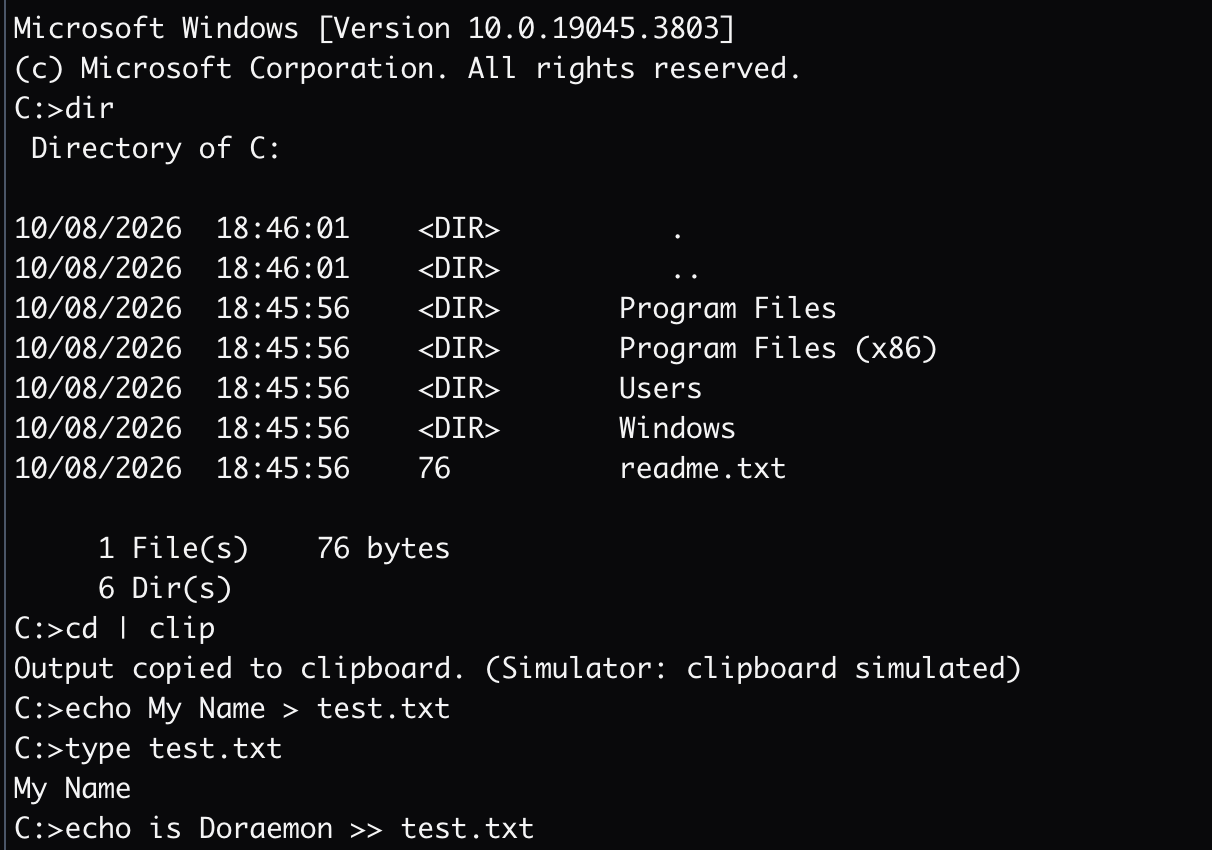
\includegraphics[keepaspectratio,alt={Example Output}]{images/wind_sim_cl_work.png}}
\caption{Example Output}
\end{figure}

\emph{Note: Since I lack a Windows device, a online simulator has been
used.}

\subsubsection{1.2 Commands in Factsheet}\label{commands-in-factsheet}

\begin{Shaded}
\begin{Highlighting}[]
\ExtensionTok{del}\NormalTok{ /p }
\CommentTok{\#same /p as before but specifically for del {-}{-} confirms Y/N before deleting ech file, not force delete }
\BuiltInTok{exit} 
\CommentTok{\#closes the terminal session}
\FunctionTok{dir}\NormalTok{ /w }
\CommentTok{\#lists contents in wide format, squeezes more names per line so less detail}
\FunctionTok{dir}\NormalTok{ /b }
\CommentTok{\#bare format (names only), no dates/sizes/etc}
\BuiltInTok{echo}\NormalTok{ \%cd\% }
\CommentTok{\#prints current folder path as text }
\FunctionTok{more}\NormalTok{ filename }
\CommentTok{\#views file page by page, pauses at each screen }
\ExtensionTok{python} 
\CommentTok{\#launches Python interpreter if installed}
\ExtensionTok{wgnuplot} 
\CommentTok{\#launches Gnuplot for plotting if installed}
\ExtensionTok{where}\NormalTok{ python }
\CommentTok{\#finds the filepath of the installed python.exe}
\end{Highlighting}
\end{Shaded}

\begin{figure}
\centering
\pandocbounded{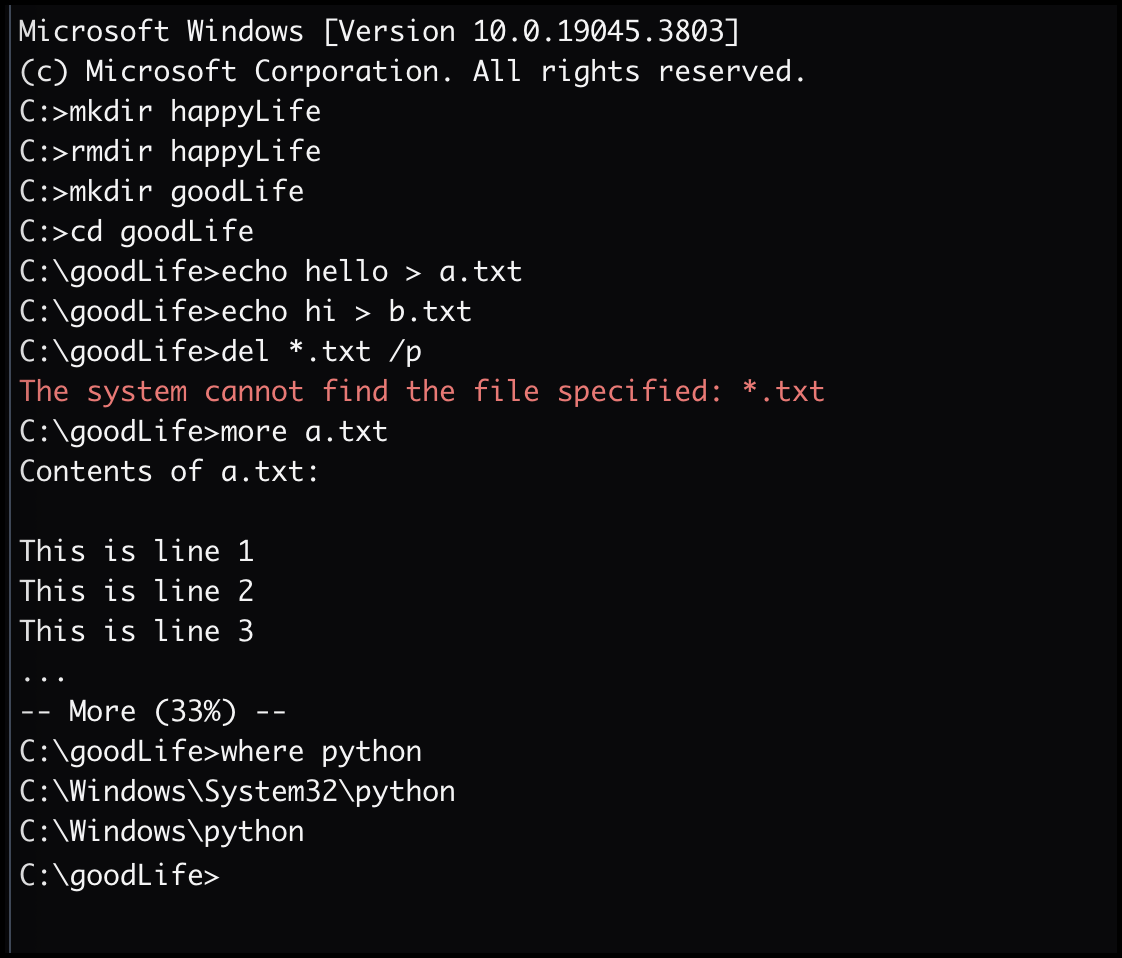
\includegraphics[keepaspectratio,alt={Sample Output on Simulator}]{images/wind_sim_fct.png}}
\caption{Sample Output on Simulator}
\end{figure}

\emph{Note: It is worth mentioning I couldn't run all the outputs on a
simulator. However the tasks in section two were performed on a real
Windows machine last week hence are realistic.}

\subsection{2. Commands and Outputs}\label{commands-and-outputs}

\subsubsection{\texorpdfstring{2.1 \ul{Task 1: Directory creation and
verification}}{2.1 Task 1: Directory creation and verification}}\label{task-1-directory-creation-and-verification}

\begin{Shaded}
\begin{Highlighting}[]
\BuiltInTok{cd}\NormalTok{ PHY134SEM12026 }
\FunctionTok{mkdir}\NormalTok{ CLI\_DOS\_July2026 }
\BuiltInTok{cd}\NormalTok{ CLI\_DOS\_July2026 dir /p}
\end{Highlighting}
\end{Shaded}

\begin{figure}
\centering
\pandocbounded{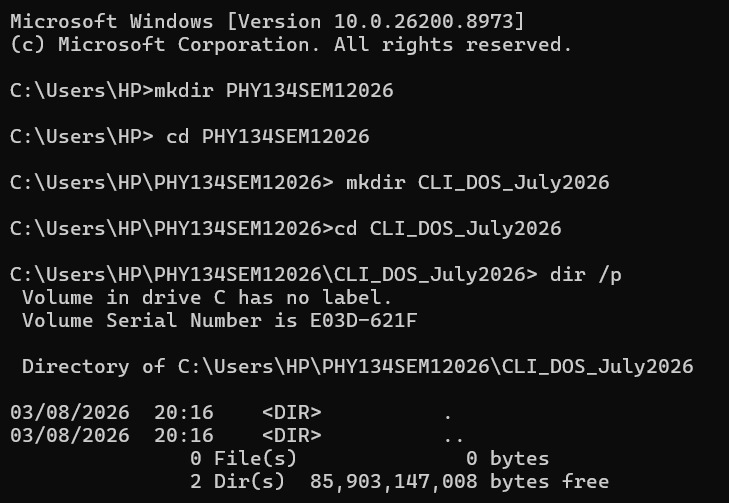
\includegraphics[keepaspectratio,alt={Task 1}]{images/Task1.jpeg}}
\caption{Task 1}
\end{figure}

\subsubsection{\texorpdfstring{2.2 \ul{Task 2: File
creation}}{2.2 Task 2: File creation}}\label{task-2-file-creation}

\begin{Shaded}
\begin{Highlighting}[]
\BuiltInTok{echo}\NormalTok{ CLI DOS Experiment Notes }\OperatorTok{\textgreater{}}\NormalTok{ notes.txt }
\BuiltInTok{type}\NormalTok{ notes.txt }
\FunctionTok{more}\NormalTok{ notes.txt }
\end{Highlighting}
\end{Shaded}

\begin{figure}
\centering
\pandocbounded{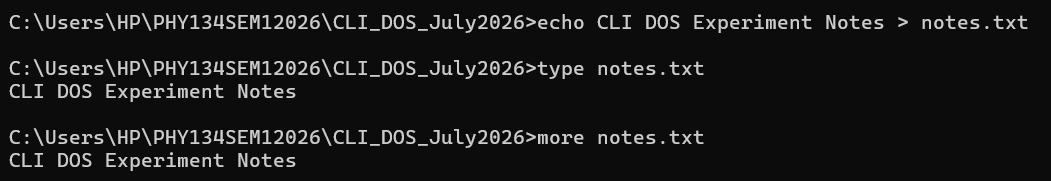
\includegraphics[keepaspectratio,alt={Task 2}]{images/Task2.jpeg}}
\caption{Task 2}
\end{figure}

\subsubsection{\texorpdfstring{2.3 \ul{Task 3: File
Relocation}}{2.3 Task 3: File Relocation}}\label{task-3-file-relocation}

\begin{Shaded}
\begin{Highlighting}[]
\FunctionTok{mkdir}\NormalTok{ Data move notes.txt Data }
\BuiltInTok{cd}\NormalTok{ Data dir }
\BuiltInTok{cd}\NormalTok{ .. }
\end{Highlighting}
\end{Shaded}

\begin{figure}
\centering
\pandocbounded{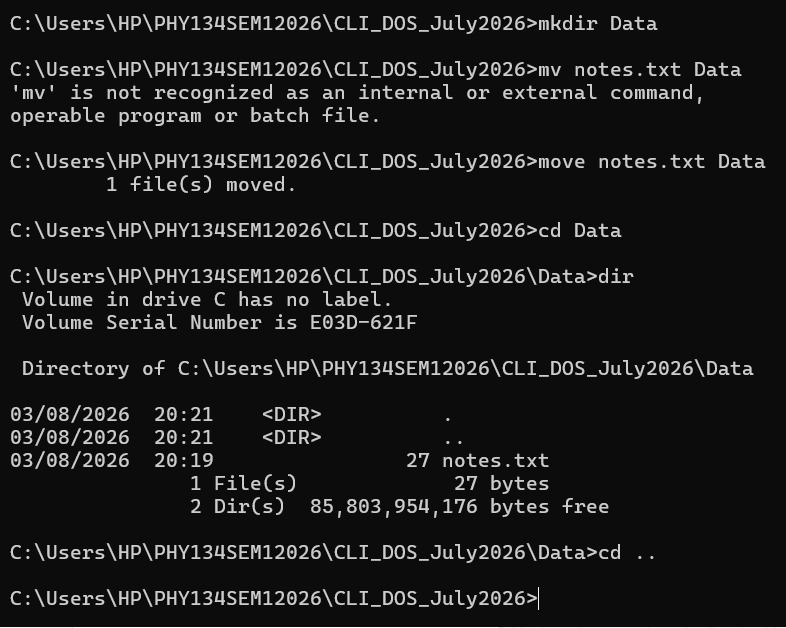
\includegraphics[keepaspectratio,alt={Task 3}]{images/Task3.jpeg}}
\caption{Task 3}
\end{figure}

\subsubsection{\texorpdfstring{2.4 \ul{Task 4: System Diagnostics
Script}}{2.4 Task 4: System Diagnostics Script}}\label{task-4-system-diagnostics-script}

\begin{Shaded}
\begin{Highlighting}[]
\BuiltInTok{type}\NormalTok{ system\_report.txt}
\end{Highlighting}
\end{Shaded}

\begin{figure}
\centering
\pandocbounded{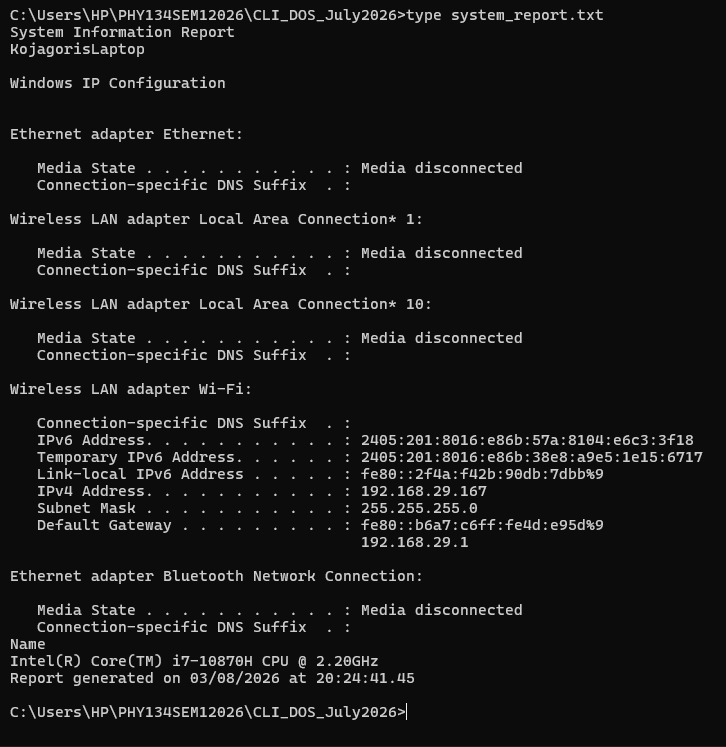
\includegraphics[keepaspectratio,alt={Task 4}]{images/Task4.jpeg}}
\caption{Task 4}
\end{figure}

\subsubsection{\texorpdfstring{2.5 \ul{Task 5: Txt File Creation and
update}}{2.5 Task 5: Txt File Creation and update}}\label{task-5-txt-file-creation-and-update}

\begin{Shaded}
\begin{Highlighting}[]
\BuiltInTok{echo}\NormalTok{ Test File }\OperatorTok{\textgreater{}}\NormalTok{ test.txt}
\BuiltInTok{echo}\NormalTok{ Updated on \%DATE\% }\OperatorTok{\textgreater{}\textgreater{}}\NormalTok{ test.txt}
\ExtensionTok{cls}
\end{Highlighting}
\end{Shaded}

\begin{figure}
\centering
\pandocbounded{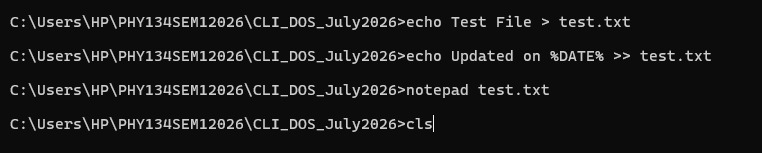
\includegraphics[keepaspectratio,alt={Task 5}]{images/Task5.jpeg}}
\caption{Task 5}
\end{figure}

\subsubsection{\texorpdfstring{2.6 \ul{Task 6: sin(x)
Plotting}}{2.6 Task 6: sin(x) Plotting}}\label{task-6-sinx-plotting}

\begin{Shaded}
\begin{Highlighting}[]
\BuiltInTok{cd}\NormalTok{ gnuplot }
\StringTok{"C:\textbackslash{}Program Files\textbackslash{}gnuplot\textbackslash{}bin\textbackslash{}gnuplot.exe"} 
\ExtensionTok{plot}\NormalTok{ sin}\ErrorTok{(}\ExtensionTok{x}\KeywordTok{)}
\end{Highlighting}
\end{Shaded}

\begin{figure}
\centering
\pandocbounded{
\includegraphics[keepaspectratio,alt={Task 6 - Script}]{images/Task6.jpeg}}
\caption{Task 6 - Script}
\end{figure}

\begin{figure}
\centering
\pandocbounded{
\includegraphics[keepaspectratio,alt={Task 6 - Plot}]{images/Task6_gnu.jpeg}}
\caption{Task 6 - Plot}
\end{figure}

\subsubsection{\texorpdfstring{2.7 \ul{Task 7: Directory
listing}}{2.7 Task 7: Directory listing}}\label{task-7-directory-listing}

\begin{Shaded}
\begin{Highlighting}[]
\FunctionTok{dir}\NormalTok{ /b }\OperatorTok{\textgreater{}}\NormalTok{ bare\textbackslash{}\_list.txt }
\FunctionTok{more}\NormalTok{ bare}\DataTypeTok{\textbackslash{}\_}\NormalTok{list.txt}
\end{Highlighting}
\end{Shaded}

\begin{figure}
\centering
\pandocbounded{
\includegraphics[keepaspectratio,alt={Task 7}]{images/Task7.jpeg}}
\caption{Task 7}
\end{figure}

\subsection{3. Experience (Workspace setup,
MacOS)}\label{experience-workspace-setup-macos}

Since I am on a machine running MacOS, the process of installation
differs vastly from the one in Windows.

Firstly, the command-line package manager for MacOS isn't one
distributed by Apple natively so you can use any of the free ones found
online. I use \texttt{brew} and
\texttt{brew\ install\ \textless{}package\textgreater{}} manages
fetch/install/updates without manual intervention.

The packages notably mentioned in Lab to be installed included:

\begin{itemize}
\tightlist
\item
  pandoc
\item
  Imagemagick
\item
  GnuPlot
\item
  Python
\end{itemize}

\subsubsection{3.1 About Python}\label{about-python}

It is worth noting that instead of using the native \texttt{pip}
globally, I prefer creating a virtual environment per project and
locally install any module I need. This is a precaution against certain
dependency conflicts (like different projects needing different
versions) that I have faced in the past and a certain
\texttt{error:\ externally-managed-environment} too.

\subsubsection{3.2 About MarkText}\label{about-marktext}

This was the one suggested in the lab however the version for MacOS is
depreciated and hence I switched to using \texttt{VSCode} with proper
extensions. Also, worth mentioning, I used the \texttt{xelatex} renderer
with pandoc since I had used that before and already had a compatible
yaml template.

\begin{figure}
\centering
\pandocbounded{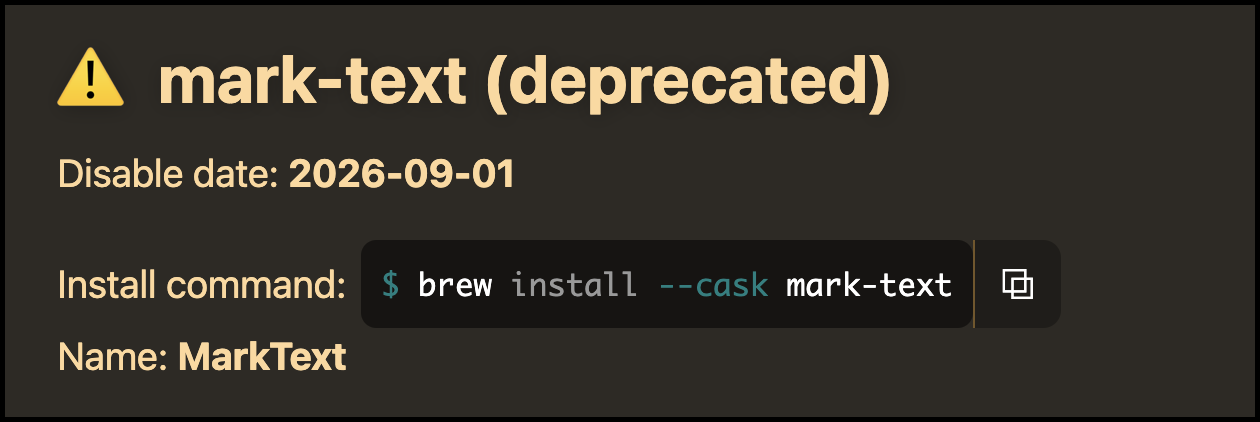
\includegraphics[keepaspectratio,alt={Depreciation Message}]{images/mark-text.png}}
\caption{Depreciation Message}
\end{figure}

\subsection{4. Conclusion}\label{conclusion}

The advantage of CLI (vs GUI) compounds as the number of files and
folders grows when in comparison, the GUI equivalent gets slower, boring
and more error-prone as scale increases.

Beyond speed, the CLI (unlike GUI) allows repeating the exact same
commands very easily. In MacOS, for example, you could press
\texttt{Ctrl+R} and repeat any command from history, eliminating the
need for retyping. This distinction matters greatly since one does not
get the matter at hand succesfully at first go most of the times.

\end{document}
